\section{Methodology}

The dataset for this study is available at \textcolor{red}{SITE}, which involves the collection of 227 gravity stations \textcolor{red}{FIGURE}. The Gravity measurements were obtained using a Lacoste and Romberg gravimeter (model G, ±0.01 mGal), while orthometric altitude was determined using a Differential Global Positioning System (DGPS) device (± 0.3 m). Data on gravity were collected at varying intervals: (i) detailed: with one station approximately every 0.3 km, forming three profiles intersecting the SAIC \textcolor{red}{FIGURE}, two traversing each lobe, and one along the internal shear zone. (ii) regional: in the country rocks, the data coverage was approximately one station per 4 km, aiming to complement the existing regional gravity dataset. This dataset was processed and interpreted in a conventional manner by xxx et al., 2021. However, in this study, we will reprocess it to perform all gravity reductions relative to the ellipsoid, thus obtaining the gravity disturbance.






\begin{figure}[tb!]
  \centering
  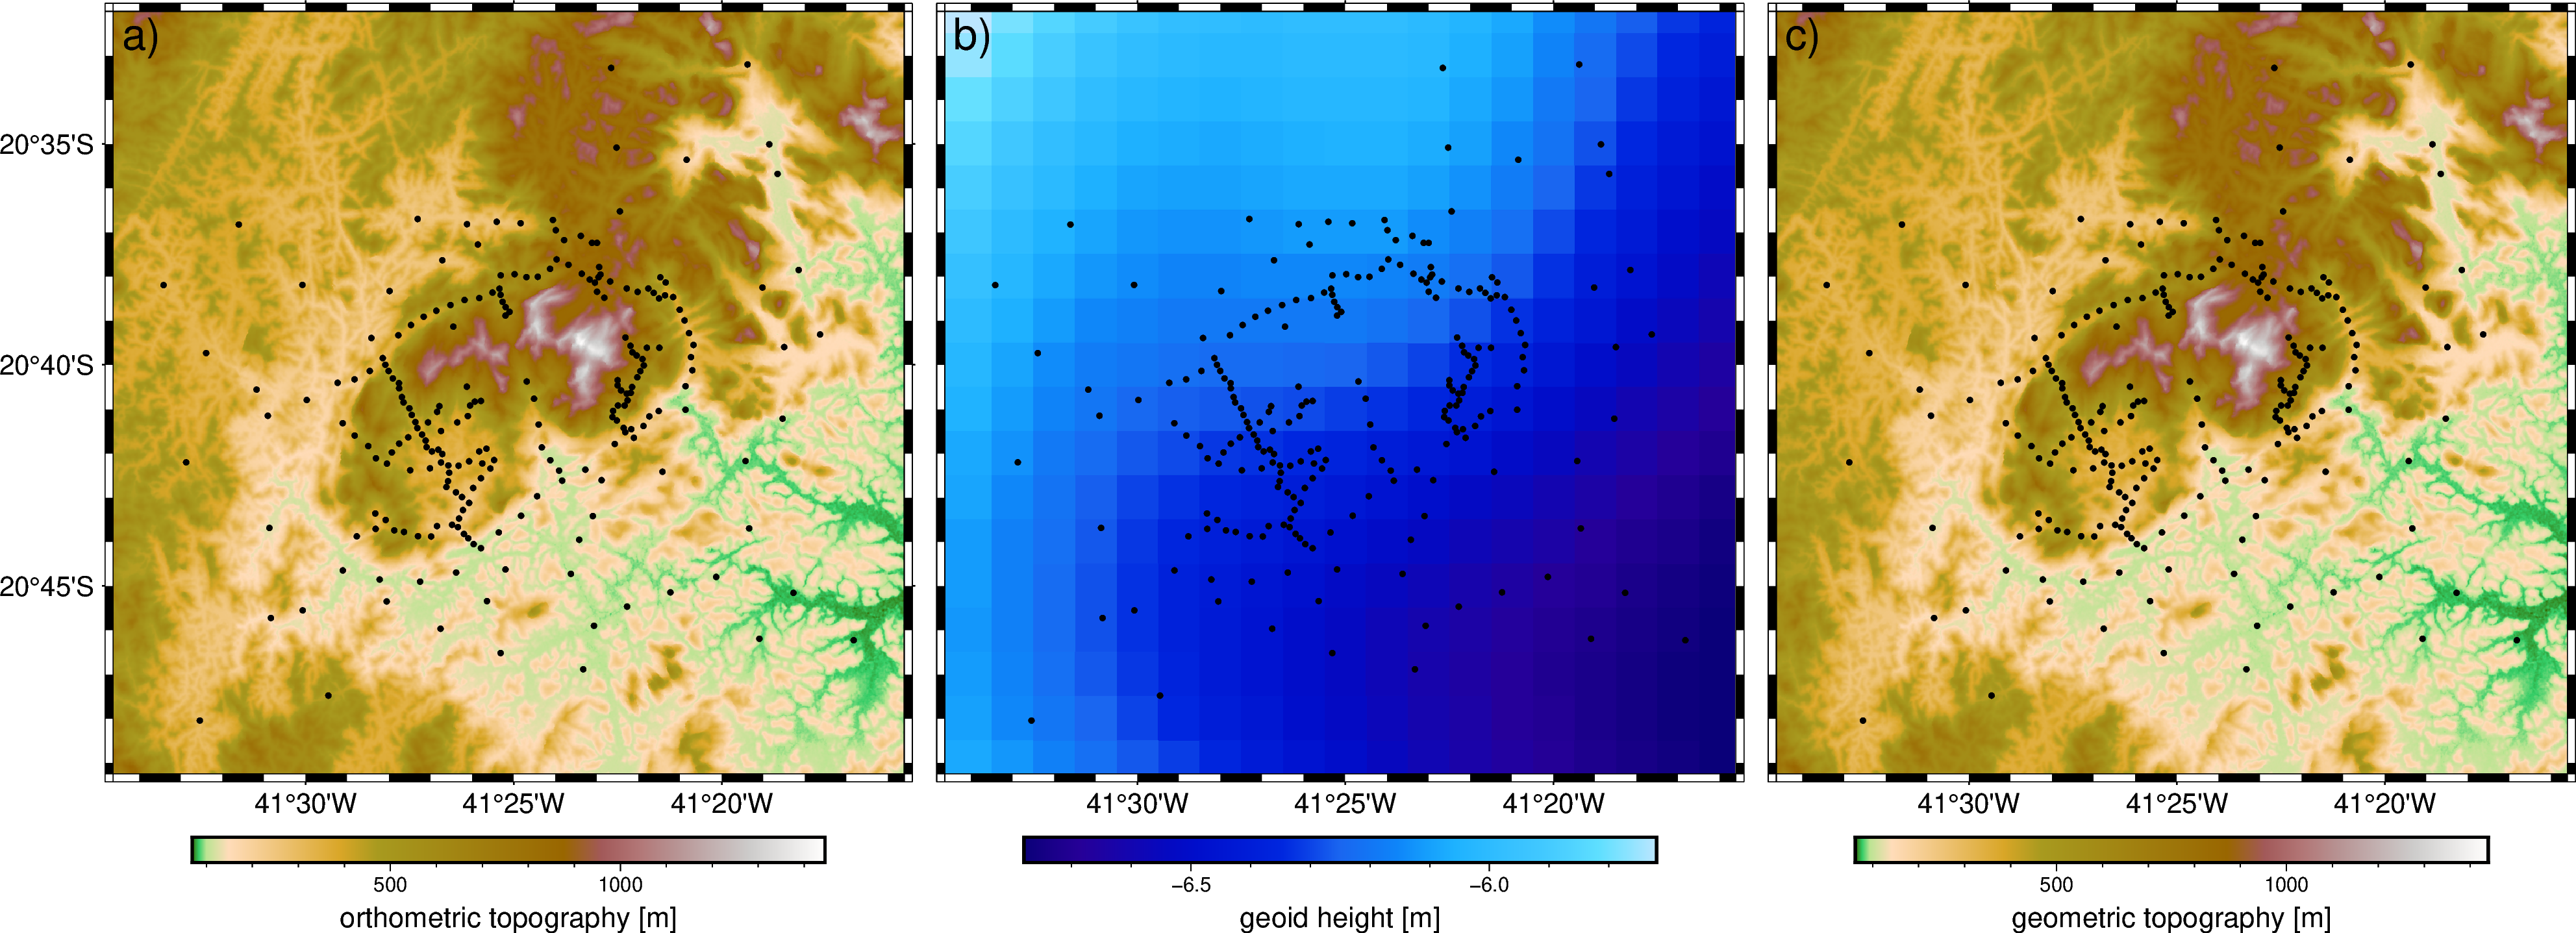
\includegraphics[width=1\linewidth]{figures/heights.png}
  \caption{
    % Addressing computational challenges in magnetic microscopy with extensive datasets.
    % a) Complete synthetic dataset featuring all N observation points including areas lacking relevant information.
    % b) Streamlining data through pre-selected windows reduces the dataset size for inversion, ensuring efficiency without compromising final results.
      }
  \label{euler1}
\end{figure}
